\section{}
Στην άσκηση αυτή θέλουμε να διαβάζουμε 2 πλήκτρα από το πληκτρολόγιο (τα 0 και
7) και μόνο τότε να ανάβουμε τα leds PA0-7, ανεξάρτητα από την χρονική
διάρκεια που έμεινε πατημένο το κάθε πλήκτρο . Ουσιαστικά πραγματοποιούμε μία
ηλεκτρονική κλειδαριά.  Εν προκειμένω, καταρχάς διαβάζουμε για να δούμε αν
έχει έρθει χαρακτήρας από το πληκτολόγιο. Αν όχι περιμένουμε έως ότου
διαβάσουμε.  Σε περίπτωση που διαβάσουμε ελέγχουμε αν είναι ο σωστός
χαρακτήρας, καταρχάς το '0' του πληκτρολογίου, το οποίο αντιστοιχεί στο hex 2.
Αν δεν είναι τότε πρέπει να περιμένουμε από την αρχή να διαβάσουμε πάλι το
'0'. Σε περίπτωση που το διαβάσουμε τότε ελεχουμε για το αν διαβάσαμε '7', το
οποίο αντιστοιχεί στο hex 10. Αν δεν διαβάσουμε το '7', τότε πάμε πάλι στην
αρχή και περιμένουμε να διαβάσουμε πάλι το first\_key (δηλαδή το '0').  Αν
διαβάσουμε επιτυχώς και τα 2 κλειδιά τότε ανάβουμε τα leds PA0-7. Παρακάτω
φαίνεται το διάγραμμα ροής και ο κώδικας.

\begin{figure}[H]
	\centering
	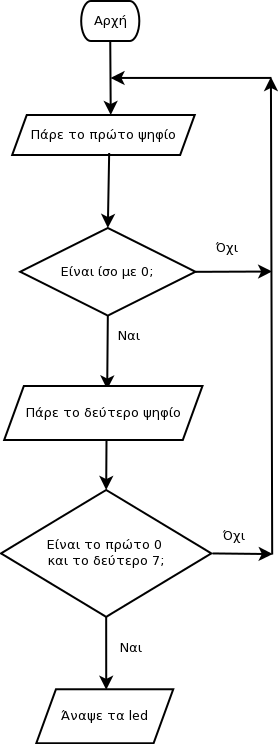
\includegraphics[height=0.5\textheight]{files/flowchart.png}
	\caption{Διάγραμμα ροής}
\end{figure}

\noindent Κυρίως κώδικας:
\inputminted[linenos,obeytabs,fontsize=\footnotesize]{c}{files/part3.S}
